\chapter{Instruction Level Parallelism (ILP)}

\section{Introduzione}
I processori con architettura pipeline sfruttano il parallelismo esistente tra le istruzioni, noto come \textbf{Instruction-Level Parallelism (ILP)}, che permette la loro esecuzione in parallelo. 
L'obiettivo principale della progettazione di queste architetture è aumentare la quantità di istruzioni diverse che vengono eseguite simultaneamente nelle diverse fasi della pipeline. Più è alta la quantità di ILP che può essere trovata e sfruttata, migliori saranno le prestazioni (performance) della pipeline.

\section{Approcci allo sfruttamento dell'ILP}
Esistono fondamentalmente due approcci per sfruttare l'ILP per evitare o mitigare i problemi derivanti dalle dipendenze di dato e dagli hazard strutturali o di controllo:

\begin{itemize}
    \item \textbf{Approccio Dinamico (Hardware-based):} È l'hardware stesso a localizzare il parallelismo in fase di esecuzione (es. architettura Tomasulo). Domina i mercati desktop e server ed è presente in processori molto spinti (es. Intel Core Series, ARM Cortex-A9, MIPS R10000/12000, RISC-V avanzati).
    \item \textbf{Approccio Statico (Software-based):} È definito dal compilatore prima dell'esecuzione. Trovava grande utilizzo in passato e domina ancora nel mercato dei sistemi \textit{embedded} (es. ARM Cortex-A8) poiché non richiedono elaborazioni hardware così spinte. Il ruolo del "compilatore" in questo contesto sarà svolto da noi, operando scelte strategiche sul codice Assembly.
\end{itemize}
I due approcci possono anche essere parzialmente combinati.

\section{Parallelismo nei Basic Block}
Per parlare di parallelizzazione statica, dobbiamo partire dal concetto fondamentale di \textit{Basic Block}. Il primo tipo di ILP si cerca tra le istruzioni che appartengono allo stesso blocco base.

\begin{definition}[Basic Block]
Un \textit{basic block} è una sequenza compatta di istruzioni che presenta le seguenti caratteristiche:
\begin{itemize}
    \item Non ha salti in ingresso, se non il punto di ingresso al blocco stesso.
    \item Non ha salti in uscita, se non il punto di uscita dal blocco.
\end{itemize}
In altre parole, nessuna istruzione entra in un punto intermedio e nessuna esce in un punto intermedio.
\end{definition}

% FIGURA DA INSERIRE QUI
% Fonte: Slide 6
% Descrizione: Diagramma a blocchi generico di un Basic Block con una singola freccia in ingresso e una in uscita.
\begin{figure}[H]
    \centering
    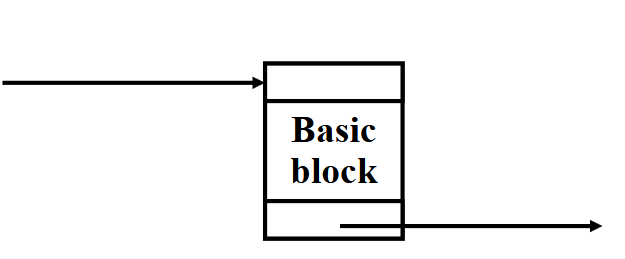
\includegraphics[width=0.4\textwidth]{capitoli/08_ILP/images/basic_block_generic.png}
    \caption{Struttura concettuale di un Basic Block.}
    \label{fig:basic_block_generic}
\end{figure}

\begin{example}
Consideriamo il seguente frammento di codice ad alto livello in C:
\begin{verbatim}
while (save[i] == k)
    i += 1;
\end{verbatim}
Il compilatore trasforma questo frammento in Assembly. Il codice risultante può essere suddiviso in due Basic Block, uno contenente le operazioni di caricamento e confronto (accesso alla memoria \texttt{save[i]} e branch), e uno contenente l'incremento dell'indice e il salto incondizionato.
\end{example}

% FIGURA DA INSERIRE QUI
% Fonte: Slide 7
% Descrizione: Codice C, codice Assembly RISC-V corrispondente e il control flow graph che mostra la suddivisione in Block 1 e Block 2.
\begin{figure}[H]
    \centering
    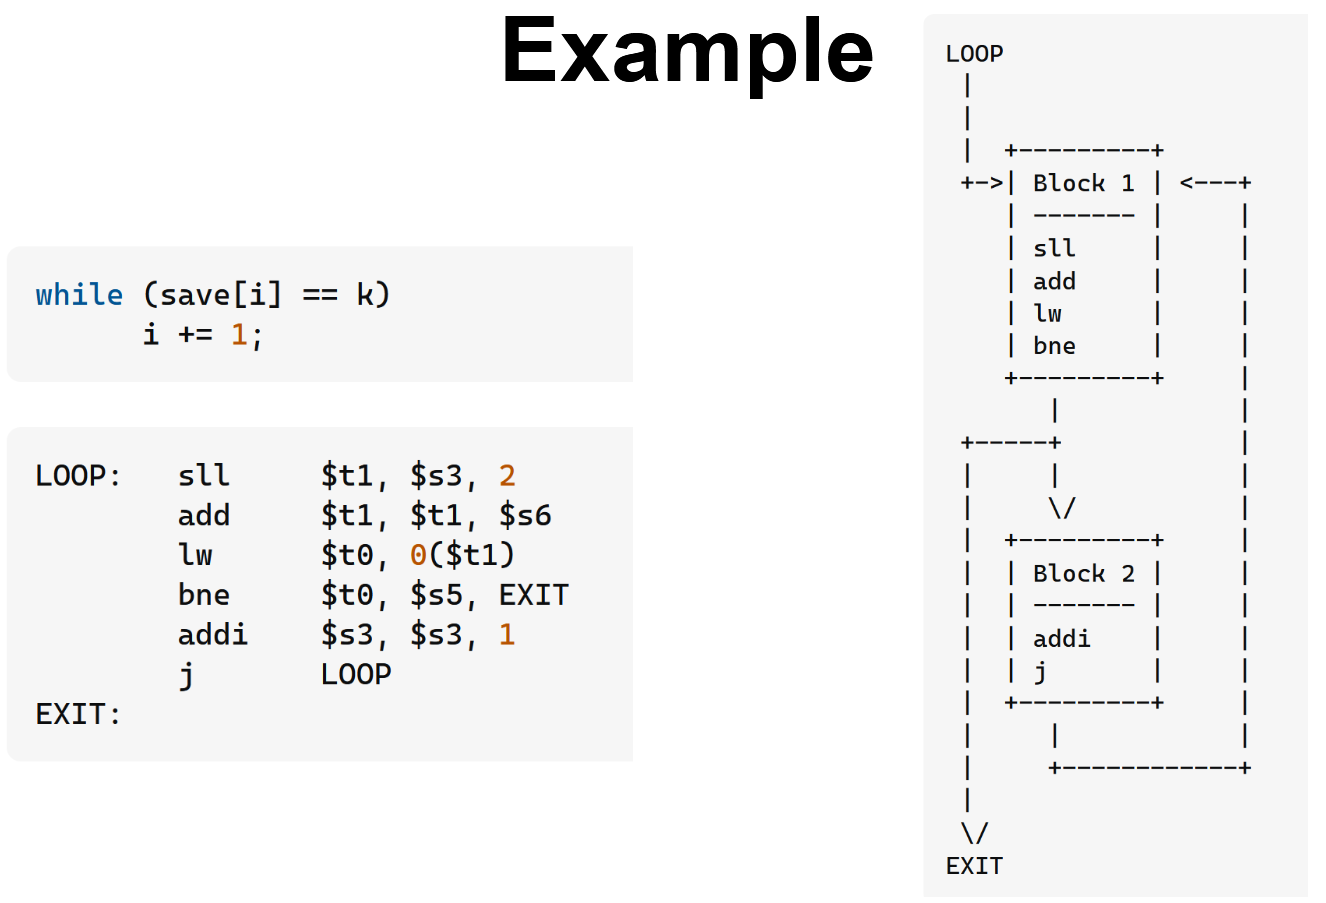
\includegraphics[width=0.7\textwidth]{capitoli/08_ILP/images/basic_block_example}
    \caption{Esempione di suddivisione del codice in Basic Blocks.}
    \label{fig:basic_block_example}
\end{figure}

\begin{remark}
\textbf{Il limite dei Basic Block:} Per i tipici programmi RISC-V, la dimensione di un basic block è molto piccola, solitamente tra le 4 e le 7 istruzioni. Poiché è altamente probabile che queste poche istruzioni siano dipendenti l'una dall'altra, la quantità di parallelismo sfruttabile all'interno di un singolo blocco base è normalmente piuttosto ridotta.
\end{remark}

\section{Tecniche di Ottimizzazione Statica (Software)}

\subsection{Rescheduling (Rischedulazione)}
All'interno di un basic block, il compilatore (o il programmatore) può rischedulare, ovvero spostare in una posizione diversa, le istruzioni per ottimizzare il codice ed evitare stalli dovuti a dipendenze di dato reali (es. dati necessari non ancora pronti a causa di latenze della memoria).

\begin{example}
Vogliamo eseguire le seguenti due operazioni ad alto livello:
\[ a = b + c; \quad d = e - f; \]
Assumiamo che le istruzioni di \texttt{load} abbiano una latenza di un colpo di clock.
Supponendo che i registri base da \texttt{x10} a \texttt{x15} siano già stati impostati, il codice Assembly non ottimizzato sarebbe:

\begin{verbatim}
lw x1, 0(x10)
lw x2, 0(x11)
add x5, x1, x2  // Dipendenza da x2 e x1
sw x5, 0(x14)
lw x3, 0(x12)
lw x4, 0(x13)
add x6, x3, x4  // Dipendenza da x4 e x3
sw x6, 0(x15)
\end{verbatim}
\end{example}

Se analizziamo l'evoluzione in pipeline di questo codice non ottimizzato, notiamo una dipendenza: \texttt{x2} è destinazione di una \texttt{load} e sorgente della \texttt{add} immediatamente successiva. Essendo \texttt{x2} disponibile solo dopo la fase \texttt{MEM}, la \texttt{add} deve stallare in fase di decodifica, facendo perdere cicli di clock. Questo si ripete per la seconda operazione. Il programma richiede \textbf{14 colpi di clock}.

Per evitare questo, applichiamo il \textbf{rescheduling}: spostiamo le \texttt{load} della seconda operazione in alto, prima delle operazioni aritmetiche, riempiendo così gli stalli (visto che si tratta di calcoli indipendenti).

\begin{table}[H]
    \centering
    \begin{tabular}{ll}
        \textbf{Codice Non Ottimizzato} & \textbf{Codice Rischedulato} \\
        \midrule
        \texttt{lw x1, 0(x10)} & \texttt{lw x1, 0(x10)} \\
        \texttt{lw x2, 0(x11)} & \texttt{lw x2, 0(x11)} \\
        \texttt{add x5, x1, x2} \textit{ (stallo)} & \texttt{lw x3, 0(x12)} \\
        \texttt{sw x5, 0(x14)} & \texttt{add x5, x1, x2} \\
        \texttt{lw x3, 0(x12)} & \texttt{lw x4, 0(x13)} \\
        \texttt{lw x4, 0(x13)} & \texttt{sw x5, 0(x14)} \\
        \texttt{add x6, x3, x4} \textit{ (stallo)}& \texttt{add x6, x3, x4} \\
        \texttt{sw x6, 0(x15)} & \texttt{sw x6, 0(x15)} \\
    \end{tabular}
    \caption{Confronto tra codice non ottimizzato e ottimizzato tramite rescheduling.}
\end{table}

\begin{figure}[H]
    \centering
    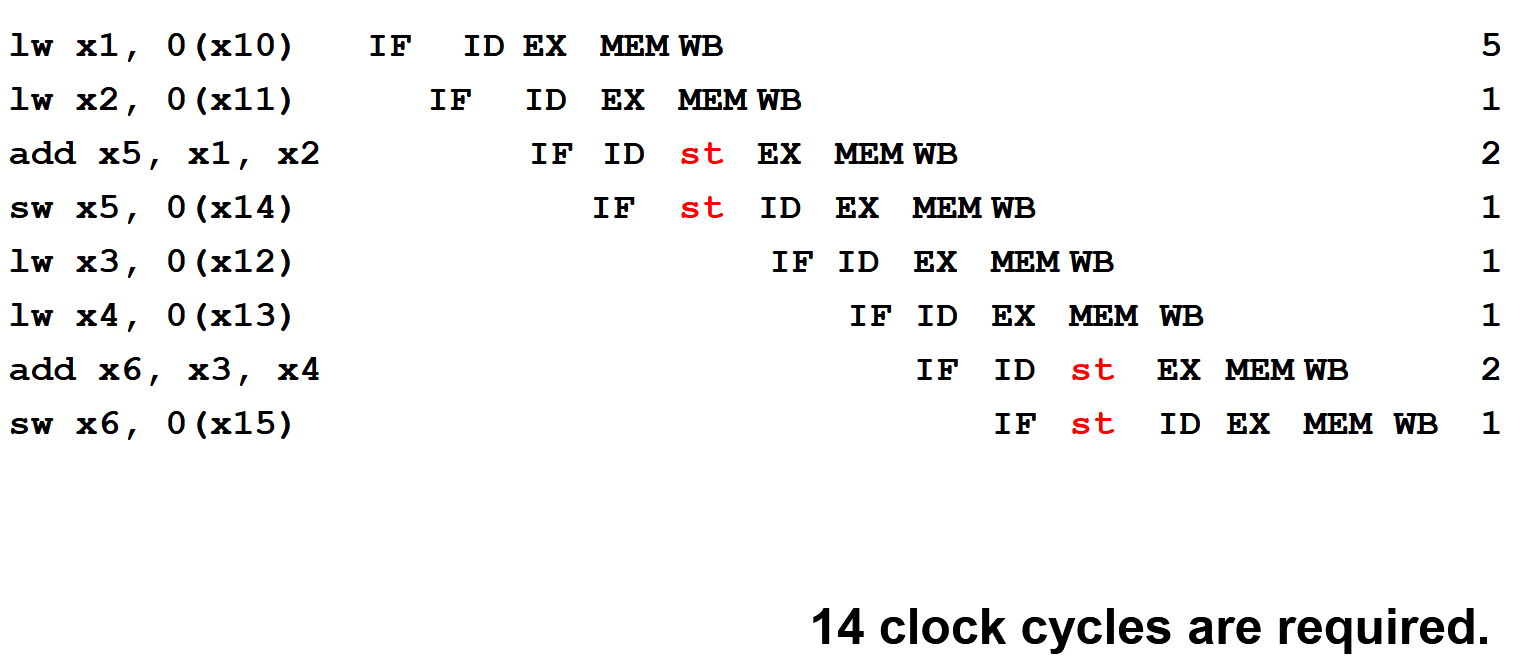
\includegraphics[width=0.5\textwidth]{capitoli/08_ILP/images/non_rescheduling_example.png}
    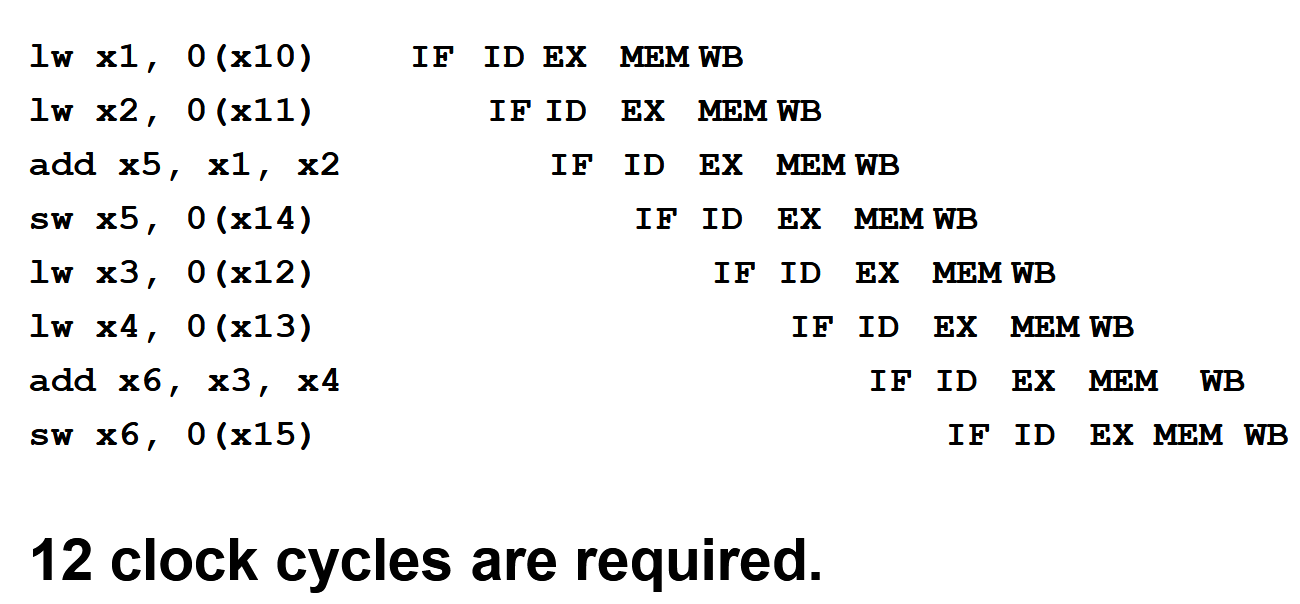
\includegraphics[width=0.5\textwidth]{capitoli/08_ILP/images/rescheduling_example.png}
    \caption{Evoluzione in pipeline del codice rischedulato, mostrando l'eliminazione degli stalli.}
    \label{fig:rescheduling_example}
\end{figure}

Con il codice rischedulato, nessun \texttt{load stall} è richiesto, e l'esecuzione si conclude in \textbf{12 colpi di clock}, risparmiando tempo prezioso.

\subsection{Loop-Level Parallelism e Loop Unrolling}
Per incrementare ulteriormente il parallelismo disponibile, non ci si ferma al singolo Basic Block (troppo piccolo), ma si considera il parallelismo tra iterazioni di un ciclo (\textit{loop}).
Due modi principali per farlo sono:
\begin{enumerate}
    \item \textbf{SIMD (Single Instruction, Multiple Data):} Usato da processori vettoriali e GPU, dove diverse unità funzionali eseguono task simili in parallelo su dati multipli con un singolo colpo di clock.
    \item \textbf{Loop Unrolling (Srotolamento dei cicli):} Tecnica (statica o dinamica) in cui il corpo del loop viene esplicitamente replicato più volte all'interno dell'iterazione.
\end{enumerate}

\begin{definition}[Loop Unrolling]
Il Loop Unrolling consiste nello srotolare un ciclo replicando il suo body. Ad esempio, invece di eseguire $N$ iterazioni saltando indietro ogni volta, si eseguono $N/4$ iterazioni contenenti ciascuna 4 repliche del body (aggiornando opportunamente gli indici e i contatori).
\end{definition}

\begin{example}
Trasformazione del ciclo in C:
\begin{verbatim}
// Ciclo Originale
for (i=0; i<N; i++) {
    x[i] = x[i] + y[i];
}

// Ciclo dopo Unrolling (fattore 4)
for (i=0; i<N; i=i+4) {
    x[i] = x[i] + y[i];
    x[i+1] = x[i+1] + y[i+1];
    x[i+2] = x[i+2] + y[i+2];
    x[i+3] = x[i+3] + y[i+3];
}
\end{verbatim}
\end{example}

\begin{remark}
\textbf{Vantaggi dell'Unrolling:} 
\begin{itemize}
    \item L'overhead relativo al controllo dell'iterazione si riduce enormemente. I salti (branch) fanno perdere colpi di clock (penalità). Se passo da 100 salti a 25 salti, sto risparmiando ben 75 colpi di clock solo in overhead di salto.
    \item Il corpo del ciclo diventa molto più ampio (creando un Basic Block "virtualmente" molto più grande), aumentando le possibilità per il compilatore di usare il \textit{rescheduling} per eliminare gli stalli.
\end{itemize}
\textbf{Svantaggi:} 
\begin{itemize}
    \item Aumenta la dimensione del codice (Code Size), poiché il corpo viene fisicamente moltiplicato in memoria.
\end{itemize}
\end{remark}

\section{Dipendenze e Hazard}
Le dipendenze sono proprietà intrinseche del programma. Esse determinano l'ordine in cui i risultati devono essere calcolati, pongono un limite superiore al parallelismo sfruttabile e creano la possibilità che si verifichi un \textit{hazard} (rischio di stallo) nell'architettura.

\subsection{Dipendenze di Dato (Data Dependencies - RAW)}
C'è una reale dipendenza di dato se il flusso di informazioni lo richiede:
\begin{itemize}
    \item l'istruzione $i$ produce un risultato che viene letto/usato dall'istruzione $j$ (Read After Write - RAW).
    \item c'è una dipendenza transitiva (es. $j$ dipende da $k$, che a sua volta dipende da $i$).
\end{itemize}

\subsection{Dipendenze di Nome (Name Dependencies)}
Si verificano quando due istruzioni utilizzano lo stesso registro o locazione di memoria (stesso \textit{nome}), ma \textbf{non esiste un reale flusso di dati} tra le due istruzioni. Creano delle "false dipendenze" che fermano inutilmente la pipeline. Si dividono in due categorie:

\subsubsection{Antidipendenza (WAR - Write After Read)}
L'istruzione $j$ \textbf{scrive} su un registro o locazione di memoria che l'istruzione $i$ \textbf{legge}, e l'istruzione $i$ deve essere eseguita prima.
\begin{example}
\begin{verbatim}
fadd.d f4, f0, f2   // i legge f0
...
fld    f0, -8(x1)   // j scrive su f0
\end{verbatim}
Non c'è flusso di dati, ma se $j$ finisse prima di $i$, modificherebbe il dato e $i$ leggerebbe un valore errato.
\end{example}

\subsubsection{Output Dependence (WAW - Write After Write)}
Sia l'istruzione $i$ che l'istruzione $j$ \textbf{scrivono} nello stesso registro o locazione di memoria. L'ordine deve essere preservato per evitare che alla fine dell'elaborazione rimanga memorizzato un valore obsoleto.

\subsection{Register Renaming (Rinominazione dei registri)}
La soluzione ai problemi creati dalle dipendenze di nome è il \textbf{Register Renaming}. Poiché non c'è flusso di dati, rinominare il registro coinvolto nella seconda istruzione "slega" completamente i due blocchi di codice, rendendoli indipendenti e parallelizzabili.
Nei processori moderni viene fatto dinamicamente in hardware; noi lo applichiamo staticamente (a mano/tramite compilatore) sfruttando i numerosi registri a disposizione (es. i 32 registri del RISC-V o i registri Floating Point).

\begin{example}
Consideriamo il seguente codice con una \textbf{Antidipendenza} (su \texttt{f6}):
\begin{verbatim}
fdiv.d f0, f2, f4
fadd.d f6, f0, f8   <-- Legge f6 per future operazioni (Output dep.) e lo scrive
fsd    f6, 0(x1)
fsub.d f8, f10, f14 
fmul.d f6, f10, f8  <-- Antidipendenza su f8 (letto sopra) e Output dep. su f6
\end{verbatim}

La \texttt{fdiv.d} è lenta. Senza accorgimenti, la \texttt{fmul.d} rischia di concludersi prima e sporcare \texttt{f6} prima che le operazioni in alto siano concluse (o viceversa). 
\textbf{Soluzione:} Sostituiamo \texttt{f6} con un registro temporaneo \texttt{S} nelle prime operazioni, eliminando la dipendenza di Output (WAW).
\begin{verbatim}
fdiv.d f0, f2, f4
fadd.d S, f0, f8   <-- Registro rinominato in S
fsd    S, 0(x1)    <-- Registro rinominato in S
fsub.d f8, f10, f14
fmul.d f6, f10, f8 <-- Ora questo blocco è indipendente
\end{verbatim}
\end{example}

\subsection{Dipendenze di Controllo}
Avvengono quando un'istruzione dipende da un salto (branch). 
\begin{remark}[Spostamento delle istruzioni rispetto ai branch]
Il professore evidenzia che quando si tenta di rischedulare spostando un'istruzione \textit{prima} o \textit{dopo} un branch per colmare uno stallo (ad esempio per riempire il \textit{branch delay slot}), bisogna prestare assoluta attenzione a due cose:
\begin{enumerate}
    \item \textbf{Data Flow:} Non modificare il flusso di dati. Se calcolo un valore prima di un salto condizionato, quel valore deve essere effettivamente utile e non andare a "sporcare" registri che serviranno in caso il salto non venga preso.
    \item \textbf{Eccezioni:} Spostare un'istruzione, come un accesso alla memoria, prima di un branch potrebbe scatenare un page fault o un cache miss su un'istruzione che in realtà il programma non avrebbe mai dovuto eseguire se il salto avesse cambiato il flusso.
\end{enumerate}
\end{remark}